\chapter{Available Deep Learning Approaches}\label{chapter: Deep Learning Approaches}

There are various approaches of autonomous driving agents making a variety of assumptions and differ in numerous options. But they can be mostly categorized into two major groups of approaches: mediated perception approaches and behavior reflex approaches. \cite{chen2015deepdriving}

In this paper we further analyse a suggested third group, called direct perception, which can traced to \cite{gibson1979ecological} in the mid 50's, but was sharply criticized by researchers of the other two groups, i.e. in \cite{ullman1980against}. %TODO: fix 60's to be the first

All these three groups differ in the way of interpreting the given sensor data and whether or not to create a some what bigger picture based on consequent data.

\section{Mediated Perception} \label{sec: Mediated Perception}

The mediated perception approach is a multi-component continuous process. Every component recognizes specific aspects for driving. For example traffic signs, lanes, other cars. Those components are then combined into one single world state representing the cars surrounding based on the sensor data. \cite{KITTI}\\
These world states are 3D models of the current world. Cars are identified using a classifier and then often surrounded by a 3D bounding box. An example can be seen in \Cref{pic: 3D Bounding Box}. By comparing different frames generated one can estimate the speed and distance to those objects and derive an A.I. based precedence behavior. \cite{KITTI}\cite{chen2015deepdriving}

The often stated problems with such approaches are, that computing such a scene is costly in terms of computation time. Some information is irrelevant, redundant or even misleading due to inaccuracy of sensors. To perform a right turn the sensor information of the distance to a car left behind me is irrelevant, but becomes very important when taking a left turn.\\
Additionally many of the subtasks are still open research topics themselves. For example a reliable lane detection throughout various weather conditions or even a new road not having any drawn lines yet. \cite{aly2008real}\\
Also mediated perception approaches require very detailed information up front, like up-to-date maps.

The approach of mediated perception is a reasonable and very sturdy way of handling such a complex task, but has its drawbacks regarding computational time and additional knowledge.

\begin{figure}
	\centering
	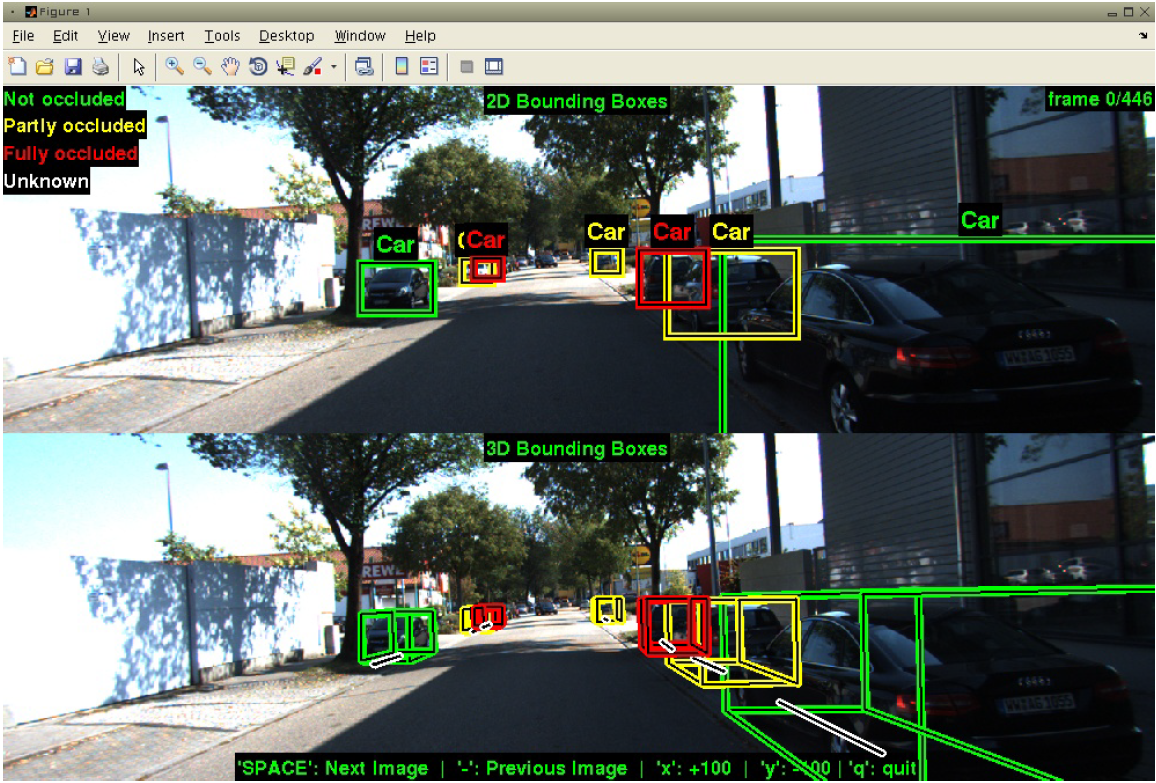
\includegraphics[scale=0.4]{src/pic/3D-boundingbox-example.png}
	\caption{An example of a scene using 3D bounding boxes. This image is taken from the MATLAB delvopment kit of \cite{KITTI}}
	\label{pic: 3D Bounding Box}
\end{figure}

\section{Behavior Reflex}\label{sec: Behavior Reflex}

The behavior reflex approach of constructing a reliable autonomous driving agent can be dated back to 1989 , where researchers tried to directly map a single frame to a decision of a steering angle. For such approaches a quite simple \nn were created. \\
The network \alvinn consisted of a single hidden layer, used back-propagation and is fed by two cameras: a $30\times32$ pixel video and a $8\times32$ pixel range finder retina. The input neurons fired depending on the blue color band of its pixel, because it is believed to infer the highest contrast between road and non-road. The difference in color of road and non-road was fed back to the network. The bias (activation level) is proportional to the proximity of the corresponding area, based on the likelihood and importance of having road in particular fields of the image.\cite{pomerleau1989alvinn}\\
For example having recognized that the road abruptly ends right in front of the car is more important than recognizing that there is a road in the top left corner.\\

Such systems, even though they are simple compared to the in \Cref{subsec: Mediated Perception} mentioned mediated perception approaches, have been proven to have the capability to perform simple tasks. It can elegantly be trained by having a human drive a car with the cameras equipped and forward the images to the \nn and adding the current steering angles as a label.\cite{chen2015deepdriving}\\

The problem with behavior reflex approaches is, that they reach their limits very early when adding more complex scenarios. Having simple alternations to the trained scenarios, which enforce a different behavior, is very hard to train to such a \nn.\\
For example comparing a simple straight 3 lane road with the car in the middle, as sketched in \Cref{fig: behavior sketches}. The system is confidently able to hold the angle and make small adjustments to stay in the lane (\Cref{fig: behavior sketches: free lane}). But what if on the same road there is an other car in the middle lane in front of the agent, which is slower? Having quite the same input the system would have to overtake the car left or right (considering an american highway) (\Cref{fig: behavior sketches: blocked lane}). Now also considering a car in front, which has the same speed. One can simple stay in the lane (\Cref{fig: behavior sketches: shared lane}). This maneuver is very hard to train to a simple \nn like \alvinn.

%\todo{noch mehr?\\}

\begin{figure}
	\centering	
	\tikzset{->,very thick,>=stealth}
	\begin{subfigure}[b]{0.32\textwidth}
		\begin{tikzpicture}[scale=0.9] % left picture
		\newcommand{\lineLength}{0.75}
		\newcommand{\lineSpace}{0.5}
		\newcommand{\startSpace}{0.25}
		
		\fill[green!50!black] (0,0) rectangle (5,5);		% background
		\fill[gray!50!black] (0.5,0) rectangle (4.5,5);     % pavement
		\fill[yellow!75!black] (0.55,0) rectangle (0.6,5);  % left yellow line
		\fill[yellow!75!black] (4.4,0) rectangle (4.45,5);  % right yellow line
		
		% left lane breaks		
		\fill[white] (1.84,\startSpace) rectangle (1.86,\lineLength+\startSpace);		
		\fill[white] (1.84,1*\lineLength + 1*\lineSpace + \startSpace) rectangle (1.86,2*\lineLength + 1*\lineSpace + \startSpace);
		\fill[white] (1.84,2*\lineLength + 2*\lineSpace + \startSpace) rectangle (1.86,3*\lineLength + 2*\lineSpace + \startSpace);
		\fill[white] (1.84,3*\lineLength + 3*\lineSpace + \startSpace) rectangle (1.86,4*\lineLength + 3*\lineSpace + \startSpace);
		
		% right line breaks
		\fill[white] (3.12,\startSpace) rectangle (3.14,\lineLength+\startSpace);		
		\fill[white] (3.12,1*\lineLength + 1*\lineSpace + \startSpace) rectangle (3.14,2*\lineLength + 1*\lineSpace + \startSpace);
		\fill[white] (3.12,2*\lineLength + 2*\lineSpace + \startSpace) rectangle (3.14,3*\lineLength + 2*\lineSpace + \startSpace);
		\fill[white] (3.12,3*\lineLength + 3*\lineSpace + \startSpace) rectangle (3.14,4*\lineLength + 3*\lineSpace + \startSpace);
		
		% cars
		\fill[red] (2.1,0.2) rectangle (2.1 + 0.8,0.2 + 1.5);
		\draw[->,very thick,  color = white] (2.5,0.4) -- (2.5,1.5);
		\draw[->,very thick,  color = green!75!black] (2.5,2) -- (2.5,3);
		
		%		\node [trapezium, minimum width = 3.6cm, trapezium angle=25,rotate = 180, opacity = 0.4, color = gray!50!white, fill] at (2.5,2) (test) {};
		%		\fill[gray!50!white, opacity = 0.4] (0.5,2.378) rectangle (4.5,5);
		\end{tikzpicture}
		\caption{free lane}
		\label{fig: behavior sketches: free lane}
	\end{subfigure}
	\begin{subfigure}[b]{0.32\textwidth}
		\begin{tikzpicture}[scale=0.9] % middle picture
		\newcommand{\lineLength}{0.75}
		\newcommand{\lineSpace}{0.5}
		\newcommand{\startSpace}{0.25}
		
		\fill[green!50!black] (0,0) rectangle (5,5);		% background
		\fill[gray!50!black] (0.5,0) rectangle (4.5,5);     % pavement
		\fill[yellow!75!black] (0.55,0) rectangle (0.6,5);  % left yellow line
		\fill[yellow!75!black] (4.4,0) rectangle (4.45,5);  % right yellow line
		
		% left lane breaks		
		\fill[white] (1.84,\startSpace) rectangle (1.86,\lineLength+\startSpace);		
		\fill[white] (1.84,1*\lineLength + 1*\lineSpace + \startSpace) rectangle (1.86,2*\lineLength + 1*\lineSpace + \startSpace);
		\fill[white] (1.84,2*\lineLength + 2*\lineSpace + \startSpace) rectangle (1.86,3*\lineLength + 2*\lineSpace + \startSpace);
		\fill[white] (1.84,3*\lineLength + 3*\lineSpace + \startSpace) rectangle (1.86,4*\lineLength + 3*\lineSpace + \startSpace);
		
		% right line breaks
		\fill[white] (3.12,\startSpace) rectangle (3.14,\lineLength+\startSpace);		
		\fill[white] (3.12,1*\lineLength + 1*\lineSpace + \startSpace) rectangle (3.14,2*\lineLength + 1*\lineSpace + \startSpace);
		\fill[white] (3.12,2*\lineLength + 2*\lineSpace + \startSpace) rectangle (3.14,3*\lineLength + 2*\lineSpace + \startSpace);
		\fill[white] (3.12,3*\lineLength + 3*\lineSpace + \startSpace) rectangle (3.14,4*\lineLength + 3*\lineSpace + \startSpace);
		
		% cars
		\fill[red] (2.1,0.2) rectangle (2.1 + 0.8,0.2 + 1.5);	% agent
		\draw[->,very thick,  color = white] (2.5,0.4) -- (2.5,1.5);
		\draw[->,very thick,  color = green!75!black] (2,1.8) -- (1.3,2.5) -- (1.3,3);
		\draw[->,very thick,  color = green!75!black] (3,1.8) -- (3.8,2.5) -- (3.8,3);
		
		
		\fill[orange] (2.1,3.2) rectangle (2.1 + 0.8,3.2 + 1.5);	% other car
		\draw[->,very thick,  color = white] (2.5,3.4) -- (2.5,4);
		\end{tikzpicture}
		\caption{slower car in the same lane}
		\label{fig: behavior sketches: blocked lane}
	\end{subfigure}
	\begin{subfigure}[b]{0.32\textwidth}
		\begin{tikzpicture}[scale=0.9] % right picture
		\newcommand{\lineLength}{0.75}
		\newcommand{\lineSpace}{0.5}
		\newcommand{\startSpace}{0.25}
		
		\fill[green!50!black] (0,0) rectangle (5,5);		% background
		\fill[gray!50!black] (0.5,0) rectangle (4.5,5);     % pavement
		\fill[yellow!75!black] (0.55,0) rectangle (0.6,5);  % left yellow line
		\fill[yellow!75!black] (4.4,0) rectangle (4.45,5);  % right yellow line
		
		% left lane breaks		
		\fill[white] (1.84,\startSpace) rectangle (1.86,\lineLength+\startSpace);		
		\fill[white] (1.84,1*\lineLength + 1*\lineSpace + \startSpace) rectangle (1.86,2*\lineLength + 1*\lineSpace + \startSpace);
		\fill[white] (1.84,2*\lineLength + 2*\lineSpace + \startSpace) rectangle (1.86,3*\lineLength + 2*\lineSpace + \startSpace);
		\fill[white] (1.84,3*\lineLength + 3*\lineSpace + \startSpace) rectangle (1.86,4*\lineLength + 3*\lineSpace + \startSpace);
		
		% right line breaks
		\fill[white] (3.12,\startSpace) rectangle (3.14,\lineLength+\startSpace);		
		\fill[white] (3.12,1*\lineLength + 1*\lineSpace + \startSpace) rectangle (3.14,2*\lineLength + 1*\lineSpace + \startSpace);
		\fill[white] (3.12,2*\lineLength + 2*\lineSpace + \startSpace) rectangle (3.14,3*\lineLength + 2*\lineSpace + \startSpace);
		\fill[white] (3.12,3*\lineLength + 3*\lineSpace + \startSpace) rectangle (3.14,4*\lineLength + 3*\lineSpace + \startSpace);
		
		% cars
		\fill[red] (2.1,0.2) rectangle (2.1 + 0.8,0.2 + 1.5);
		\draw[->,very thick,  color = white] (2.5,0.4) -- (2.5,1.5);
		\draw[->,very thick,  color = green!75!black] (2.5,2) -- (2.5,3);
		
		\fill[orange] (2.1,3.2) rectangle (2.1 + 0.8,3.2 + 1.5);	% other car
		\draw[->,very thick,  color = white] (2.5,3.4) -- (2.5,4.5);
		\end{tikzpicture}
		\caption{equal fast car in same lane}
		\label{fig: behavior sketches: shared lane}
	\end{subfigure}
	\caption{The 3 scenarios causing problems with behavior reflex approaches. The red block is the agent, the orange block the other car, the white arrows indicate the velocity and the green arrows the logically deduced behaviors.}
	\label{fig: problematic behavior sketches}
\end{figure}

%\begin{figure}
%	\centering
%	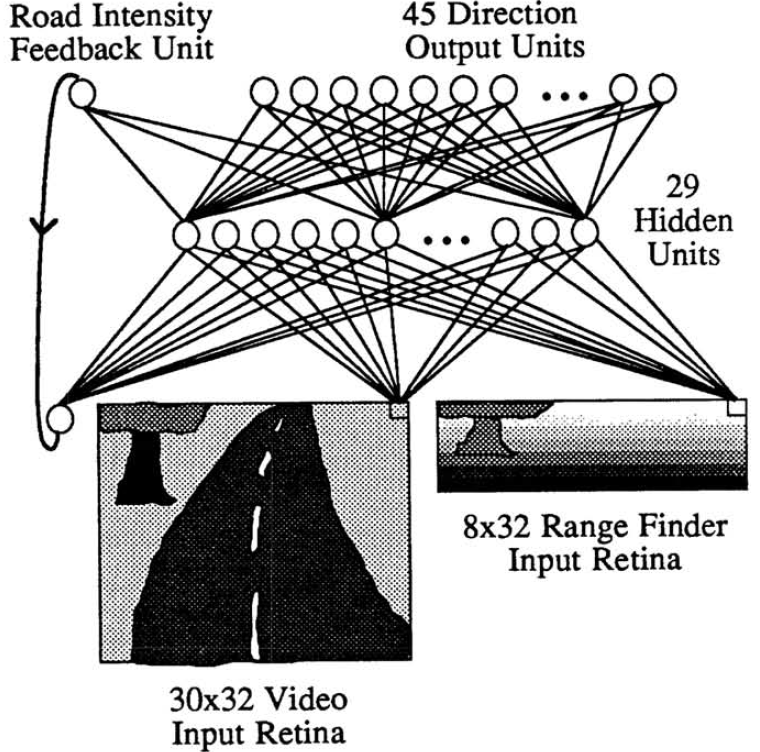
\includegraphics[scale=0.4]{src/pic/ALVINN.png}
%	\caption{The \nn called \alvinn and used as a behavior reflex based autonomous agent. \cite{pomerleau1989alvinn}}
%	\label{pic: ALVINN}
%\end{figure}

\section{Direct Perception}\label{sec: Direct Perception}

%In this paper we further analyze a suggested third group, called direct perception, which can traced to \cite{gibson2014ecological} in the late 80's, but was sharply criticized by researchers of the other two groups, i.e. in \cite{ullman1980against}.

The direct perception is the third group of approaches, which can be dated back to the 1954 and was initially mainly researched by James J. Gibson. \cite{gibson1954theory} The approach is based on analyzing a picture, not simply deducing a steering angle, or velocity change, like the behavior reflex approaches (cf. \Cref{subsec: Behavior Reflex}), but also performing further computation without parsing it into a 3D world state model like the mediated perception approaches (cf. \Cref{subsec: Mediated Perception}). \cite{chen2015deepdriving}\\
So it is a third paradigm, which can be interpreted as a hybrid of the two other paradigms. The approach tries to identify only the meaningful affordance indicators and make a decision based on those parameters. 

The CNN gets trained to make a reasonable assumption about the distance of other vehicles, their velocity and lane marks. These assumptions are further called affordance indicators.

We further consider a design based on \cite{chen2015deepdriving} and their way of training.

The original paper \cite{chen2015deepdriving} stated the a total number of 13 indicators separated in two states to be sufficient for their design of a highway only autonomous agent. The states are: in line driving (following the lane) and on line driving (changing lanes). The values themselves can be categorized as: preceding car distances, distances to the lane markers and the steering angle. The indicators and their affiliation to the states can be seen in \Cref{lst: affordance indicators}.

\begin{figure}
\centering
\todoLine
\begin{lstlisting}
always:
  1) angle: angle between the car's heading and the tangent of the road
"in lane system", when driving in the lane:
  2) toMarking LL: distance to the left lane marking of the left lane
  3) toMarking ML: distance to the left lane marking of the current lane
  4) toMarking MR: distance to the right lane marking of the current lane
  5) toMarking RR: distance to the right lane marking of the right lane
  6) dist LL: distance to the preceding car in the left lane
  7) dist MM: distance to the preceding car in the current lane
  8) dist RR: distance to the preceding car in the right lane
"on marking system", when driving on the lane marking:
  9) toMarking L: distance to the left lane marking
  10) toMarking M: distance to the central lane marking
  11) toMarking R: distance to the right lane marking
  12) dist L: distance to the preceding car in the left lane
  13) dist R: distance to the preceding car in the right lane
\end{lstlisting}

\todoLine
\caption{The affordance indicators and their affiliation states}
\label{lst: affordance indicators}
\end{figure}

Based on the current state, all affordance indicators of the other state are not used, since the other state is defined to be inactive.\\
In order to identify the current state the host car is in, every state has their respective region, where they are active with an overlapping region for smooth transitioning.

Training is done by feeding the CNN with images of a current driving scenario as input and give estimated values to the mentioned affordance indicators active in the current state. Those values get forwarded to a controller dealing with the car. In the original approach the training was done via the \torcs game further explained in TODO %TODO: ref

The controller is setup to take the affordance values and compute a decision from it in an imperative way. For example the steering can be computed as 
	$$ steerCmd = C \cdot (angle-\frac{dist\_center}{road\_width})$$
where $dist\_center$ is the center of the current state (line we are on or middle of the lane), a coefficient $C$ suited for the current conditions, like weather or speed, and $angle\in [-\pi, \pi]$ as the affordance indicator.

Also using the controller to compute the accelerating and braking one can adjust the desired speed ($desired\_speed$) based on the affordance indicators. The $desired\_speed$ is set to the speed the agent wants to drive and can drop if a drastic steering motion is considered or accelerate to overtake a slower car.\\
In a one lane scenario with a  preceding car driving slower than the $desired\_speed$ there is no space to overtake. For that the controller has the velocity control car-following model:
	$$ v(t) = v_{max}(1-e^{-\frac{c\cdot dist(t)}{v_{max}} -d})$$ 
where $v_{max}$ is the maximal speed the agent is allowed to drive, $c$ and $d$ are coefficients specific to external conditions, like a wet lane or the cars potential of accelerating and braking, and $dist(t)$ is the distance to the preceding car. This distance is given through the trained CNN.

\begin{figure}
	\centering	
	\tikzset{->,very thick,>=stealth}
	\begin{subfigure}[b]{0.32\textwidth}
		\begin{tikzpicture}[scale=0.9] % top left picture
		\newcommand{\lineLength}{0.75}
		\newcommand{\lineSpace}{0.5}
		\newcommand{\startSpace}{0.25}
		
		\fill[green!50!black] (0,0) rectangle (5,5);		% background
		\fill[gray!50!black] (0.5,0) rectangle (4.5,5);     % pavement
		\fill[yellow!75!black] (0.55,0) rectangle (0.6,5);  % left yellow line
		\fill[yellow!75!black] (4.4,0) rectangle (4.45,5);  % right yellow line
		
		% left lane breaks		
		\fill[white] (1.84,\startSpace) rectangle (1.86,\lineLength+\startSpace);		
		\fill[white] (1.84,1*\lineLength + 1*\lineSpace + \startSpace) rectangle (1.86,2*\lineLength + 1*\lineSpace + \startSpace);
		\fill[white] (1.84,2*\lineLength + 2*\lineSpace + \startSpace) rectangle (1.86,3*\lineLength + 2*\lineSpace + \startSpace);
		\fill[white] (1.84,3*\lineLength + 3*\lineSpace + \startSpace) rectangle (1.86,4*\lineLength + 3*\lineSpace + \startSpace);
		
		% right line breaks
		\fill[white] (3.12,\startSpace) rectangle (3.14,\lineLength+\startSpace);		
		\fill[white] (3.12,1*\lineLength + 1*\lineSpace + \startSpace) rectangle (3.14,2*\lineLength + 1*\lineSpace + \startSpace);
		\fill[white] (3.12,2*\lineLength + 2*\lineSpace + \startSpace) rectangle (3.14,3*\lineLength + 2*\lineSpace + \startSpace);
		\fill[white] (3.12,3*\lineLength + 3*\lineSpace + \startSpace) rectangle (3.14,4*\lineLength + 3*\lineSpace + \startSpace);
		
		% cars
		\fill[red] (2.1,0.2) rectangle (2.1 + 0.8,0.2 + 1.5);	% agent		
		\fill[orange] (0.8,3.9) rectangle (0.8 + 0.8,3.9 + 1.1);	% left other car
		\fill[orange] (2.1,2.6) rectangle (2.1 + 0.8,2.6 + 1.5);	% middle other car
		\fill[orange] (3.4,3.2) rectangle (3.4 + 0.8,3.2 + 1.5);	% right other car
		\end{tikzpicture}
		\caption{slower car in the same lane}
		\label{fig: affordance indicators: in lane - lines}
	\end{subfigure}
	\begin{subfigure}[b]{0.32\textwidth}
		\begin{tikzpicture}[scale=0.9] % top middles picture
		\newcommand{\lineLength}{0.75}
		\newcommand{\lineSpace}{0.5}
		\newcommand{\startSpace}{0.25}
		
		\fill[green!50!black] (0,0) rectangle (5,5);		% background
		\fill[gray!50!black] (0.5,0) rectangle (4.5,5);     % pavement
		\fill[yellow!75!black] (0.55,0) rectangle (0.6,5);  % left yellow line
		\fill[yellow!75!black] (4.4,0) rectangle (4.45,5);  % right yellow line
		
		% left lane breaks		
		\fill[white] (1.84,\startSpace) rectangle (1.86,\lineLength+\startSpace);		
		\fill[white] (1.84,1*\lineLength + 1*\lineSpace + \startSpace) rectangle (1.86,2*\lineLength + 1*\lineSpace + \startSpace);
		\fill[white] (1.84,2*\lineLength + 2*\lineSpace + \startSpace) rectangle (1.86,3*\lineLength + 2*\lineSpace + \startSpace);
		\fill[white] (1.84,3*\lineLength + 3*\lineSpace + \startSpace) rectangle (1.86,4*\lineLength + 3*\lineSpace + \startSpace);
		
		% right line breaks
		\fill[white] (3.12,\startSpace) rectangle (3.14,\lineLength+\startSpace);		
		\fill[white] (3.12,1*\lineLength + 1*\lineSpace + \startSpace) rectangle (3.14,2*\lineLength + 1*\lineSpace + \startSpace);
		\fill[white] (3.12,2*\lineLength + 2*\lineSpace + \startSpace) rectangle (3.14,3*\lineLength + 2*\lineSpace + \startSpace);
		\fill[white] (3.12,3*\lineLength + 3*\lineSpace + \startSpace) rectangle (3.14,4*\lineLength + 3*\lineSpace + \startSpace);
		
		% cars
		\fill[red] (2.1,0.2) rectangle (2.1 + 0.8,0.2 + 1.5);
		\fill[orange] (0.8,3.9) rectangle (0.8 + 0.8,3.9 + 1.1);	% left other car
		\fill[orange] (2.1,2.6) rectangle (2.1 + 0.8,2.6 + 1.5);	% middle other car
		\fill[orange] (3.4,3.2) rectangle (3.4 + 0.8,3.2 + 1.5);	% right other car
		\end{tikzpicture}
		\caption{equal fast car in same lane}
		\label{fig: affordance indicators: in lane - cars}
	\end{subfigure}
	\begin{subfigure}[b]{0.32\textwidth}
		\begin{tikzpicture}[scale=0.9] % top left picture
		\newcommand{\lineLength}{0.75}
		\newcommand{\lineSpace}{0.5}
		\newcommand{\startSpace}{0.25}
		
		\fill[green!50!black] (0,0) rectangle (5,5);		% background
		
%		\draw [-,gray!50!black,thick,domain=0:60] plot ({2.5*cos(\x)-1.25}, {2.5*sin(\x)});
%		\draw [-,gray!50!black,thick,domain=16:50] plot ({6.5*cos(\x)-1.25}, {6.5*sin(\x)});
%		\fill[gray!50!black] (0.5,0) rectangle (4.5,5);     % pavement
		
%		\fill[yellow!75!black] (0.55,0) rectangle (0.6,5);  % left yellow line
%		\fill[yellow!75!black] (4.4,0) rectangle (4.45,5);  % right yellow line
		
		% left lane breaks		
%		\fill[white] (1.84,\startSpace) rectangle (1.86,\lineLength+\startSpace);		
%		\fill[white] (1.84,1*\lineLength + 1*\lineSpace + \startSpace) rectangle (1.86,2*\lineLength + 1*\lineSpace + \startSpace);
%		\fill[white] (1.84,2*\lineLength + 2*\lineSpace + \startSpace) rectangle (1.86,3*\lineLength + 2*\lineSpace + \startSpace);
%		\fill[white] (1.84,3*\lineLength + 3*\lineSpace + \startSpace) rectangle (1.86,4*\lineLength + 3*\lineSpace + \startSpace);
		
		% right line breaks
%		\fill[white] (3.12,\startSpace) rectangle (3.14,\lineLength+\startSpace);		
%		\fill[white] (3.12,1*\lineLength + 1*\lineSpace + \startSpace) rectangle (3.14,2*\lineLength + 1*\lineSpace + \startSpace);
%		\fill[white] (3.12,2*\lineLength + 2*\lineSpace + \startSpace) rectangle (3.14,3*\lineLength + 2*\lineSpace + \startSpace);
%		\fill[white] (3.12,3*\lineLength + 3*\lineSpace + \startSpace) rectangle (3.14,4*\lineLength + 3*\lineSpace + \startSpace);
		
		% cars
%		\fill[red] (2.1,0.2) rectangle (2.1 + 0.8,0.2 + 1.5);
		
		%		\node [trapezium, minimum width = 3.6cm, trapezium angle=25,rotate = 180, opacity = 0.4, color = gray!50!white, fill] at (2.5,2) (test) {};
		%		\fill[gray!50!white, opacity = 0.4] (0.5,2.378) rectangle (4.5,5);
		\end{tikzpicture}
		\caption{}
		\label{fig: affordance indicators: angle}
	\end{subfigure}
	
	\begin{subfigure}[b]{0.32\textwidth}
		\begin{tikzpicture}[scale=0.9] % bottom left picture
		\newcommand{\lineLength}{0.75}
		\newcommand{\lineSpace}{0.5}
		\newcommand{\startSpace}{0.25}
		
		\fill[green!50!black] (0,0) rectangle (5,5);		% background
		\fill[gray!50!black] (0.5,0) rectangle (4.5,5);     % pavement
		\fill[yellow!75!black] (0.55,0) rectangle (0.6,5);  % left yellow line
		\fill[yellow!75!black] (4.4,0) rectangle (4.45,5);  % right yellow line
		
		% left lane breaks		
		\fill[white] (1.84,\startSpace) rectangle (1.86,\lineLength+\startSpace);		
		\fill[white] (1.84,1*\lineLength + 1*\lineSpace + \startSpace) rectangle (1.86,2*\lineLength + 1*\lineSpace + \startSpace);
		\fill[white] (1.84,2*\lineLength + 2*\lineSpace + \startSpace) rectangle (1.86,3*\lineLength + 2*\lineSpace + \startSpace);
		\fill[white] (1.84,3*\lineLength + 3*\lineSpace + \startSpace) rectangle (1.86,4*\lineLength + 3*\lineSpace + \startSpace);
		
		% right line breaks
		\fill[white] (3.12,\startSpace) rectangle (3.14,\lineLength+\startSpace);		
		\fill[white] (3.12,1*\lineLength + 1*\lineSpace + \startSpace) rectangle (3.14,2*\lineLength + 1*\lineSpace + \startSpace);
		\fill[white] (3.12,2*\lineLength + 2*\lineSpace + \startSpace) rectangle (3.14,3*\lineLength + 2*\lineSpace + \startSpace);
		\fill[white] (3.12,3*\lineLength + 3*\lineSpace + \startSpace) rectangle (3.14,4*\lineLength + 3*\lineSpace + \startSpace);
		
		% cars
		\fill[red] (1.5,0.2) rectangle (1.5 + 0.8,0.2 + 1.5);
		\fill[orange] (0.8,3.9) rectangle (0.8 + 0.8,3.9 + 1.1);	% left other car
		\fill[orange] (2.1,2.6) rectangle (2.1 + 0.8,2.6 + 1.5);	% middle other car
		\fill[gray!50!white] (3.4,3.2) rectangle (3.4 + 0.8,3.2 + 1.5);	% right other car
		%		\node [trapezium, minimum width = 3.6cm, trapezium angle=25,rotate = 180, opacity = 0.4, color = gray!50!white, fill] at (2.5,2) (test) {};
		%		\fill[gray!50!white, opacity = 0.4] (0.5,2.378) rectangle (4.5,5);
		\end{tikzpicture}
		\caption{free lane}
		\label{fig: affordance indicators: on lane - lines}
	\end{subfigure}
	\begin{subfigure}[b]{0.32\textwidth}
		\begin{tikzpicture}[scale=0.9] % bottom middle picture
		\newcommand{\lineLength}{0.75}
		\newcommand{\lineSpace}{0.5}
		\newcommand{\startSpace}{0.25}
		
		\fill[green!50!black] (0,0) rectangle (5,5);		% background
		\fill[gray!50!black] (0.5,0) rectangle (4.5,5);     % pavement
		\fill[yellow!75!black] (0.55,0) rectangle (0.6,5);  % left yellow line
		\fill[yellow!75!black] (4.4,0) rectangle (4.45,5);  % right yellow line
		
		% left lane breaks		
		\fill[white] (1.84,\startSpace) rectangle (1.86,\lineLength+\startSpace);		
		\fill[white] (1.84,1*\lineLength + 1*\lineSpace + \startSpace) rectangle (1.86,2*\lineLength + 1*\lineSpace + \startSpace);
		\fill[white] (1.84,2*\lineLength + 2*\lineSpace + \startSpace) rectangle (1.86,3*\lineLength + 2*\lineSpace + \startSpace);
		\fill[white] (1.84,3*\lineLength + 3*\lineSpace + \startSpace) rectangle (1.86,4*\lineLength + 3*\lineSpace + \startSpace);
		
		% right line breaks
		\fill[white] (3.12,\startSpace) rectangle (3.14,\lineLength+\startSpace);		
		\fill[white] (3.12,1*\lineLength + 1*\lineSpace + \startSpace) rectangle (3.14,2*\lineLength + 1*\lineSpace + \startSpace);
		\fill[white] (3.12,2*\lineLength + 2*\lineSpace + \startSpace) rectangle (3.14,3*\lineLength + 2*\lineSpace + \startSpace);
		\fill[white] (3.12,3*\lineLength + 3*\lineSpace + \startSpace) rectangle (3.14,4*\lineLength + 3*\lineSpace + \startSpace);
		
		% cars
		\fill[red] (1.5,0.2) rectangle (1.5 + 0.8,0.2 + 1.5);
		\fill[orange] (0.8,3.9) rectangle (0.8 + 0.8,3.9 + 1.1);	% left other car
		\fill[orange] (2.1,2.6) rectangle (2.1 + 0.8,2.6 + 1.5);	% middle other car
		\fill[gray!50!white] (3.4,3.2) rectangle (3.4 + 0.8,3.2 + 1.5);	% right other car
		\end{tikzpicture}
		\caption{slower car in the same lane}
		\label{fig: affordance indicators: on lane - cars}
	\end{subfigure}
	\begin{subfigure}[b]{0.32\textwidth}
		\begin{tikzpicture}[scale=0.9] % bottom right picture
		\newcommand{\lineLength}{0.75}
		\newcommand{\lineSpace}{0.5}
		\newcommand{\startSpace}{0.25}
		
		\fill[green!50!black] (0,0) rectangle (5,5);		% background
		\fill[gray!50!black] (0.5,0) rectangle (4.5,5);     % pavement
		\fill[yellow!75!black] (0.55,0) rectangle (0.6,5);  % left yellow line
		\fill[yellow!75!black] (4.4,0) rectangle (4.45,5);  % right yellow line
		
		
		% overlapping areas
		\fill[black] (1.4,0.5) rectangle (1.4+0.15,0.5 + 4);
		\fill[gray!75!black] (1.55,0.5) rectangle (1.55 + 0.6,0.5 + 4);
		\fill[black] (2.15,0.5) rectangle (2.15+0.15,0.5 + 4);
		
		\fill[black] (1.4 +1.25,0.5) rectangle (1.4+0.15 +1.25,0.5 + 4);
		\fill[gray!75!black] (1.55 + 1.25 ,0.5) rectangle (1.55 + 0.6 +1.25,0.5 + 4);
		\fill[black] (2.15 +1.25,0.5) rectangle (2.15+0.15 +1.25,0.5 + 4);
		
		% left lane breaks		
		\fill[white] (1.84,\startSpace) rectangle (1.86,\lineLength+\startSpace);		
		\fill[white] (1.84,1*\lineLength + 1*\lineSpace + \startSpace) rectangle (1.86,2*\lineLength + 1*\lineSpace + \startSpace);
		\fill[white] (1.84,2*\lineLength + 2*\lineSpace + \startSpace) rectangle (1.86,3*\lineLength + 2*\lineSpace + \startSpace);
		\fill[white] (1.84,3*\lineLength + 3*\lineSpace + \startSpace) rectangle (1.86,4*\lineLength + 3*\lineSpace + \startSpace);
		
		% right line breaks
		\fill[white] (3.12,\startSpace) rectangle (3.14,\lineLength+\startSpace);		
		\fill[white] (3.12,1*\lineLength + 1*\lineSpace + \startSpace) rectangle (3.14,2*\lineLength + 1*\lineSpace + \startSpace);
		\fill[white] (3.12,2*\lineLength + 2*\lineSpace + \startSpace) rectangle (3.14,3*\lineLength + 2*\lineSpace + \startSpace);
		\fill[white] (3.12,3*\lineLength + 3*\lineSpace + \startSpace) rectangle (3.14,4*\lineLength + 3*\lineSpace + \startSpace);
		\end{tikzpicture}
		\caption{equal fast car in same lane}
		\label{fig: affordance indicators: overlapping areas}
	\end{subfigure}
	
	\caption{The 3 scenarios causing problems with behavior reflex approaches. The red block is the agent, the orange block the other car, the white arrows indicate the velocity and the green arrows the logically deduced behaviors.}
	\label{fig: behavior sketches}
\end{figure}

\todo{\begin{enumerate}
\item show graphic of how controller computes
\end{enumerate}}

